\documentclass{article}
\usepackage[minionint,mathlf,textlf]{MinionPro} % To gussy up a bit
\usepackage[margin=1in]{geometry}
\usepackage{graphicx} % For .eps inclusion
%\usepackage{indentfirst} % Controls indentation
\usepackage[compact]{titlesec} % For regulating spacing before section titles
\usepackage{adjustbox} % For vertically-aligned side-by-side minipages
\usepackage{array, mathrsfs, mhchem, amsmath} % For centering of tabulars with text-wrapping columns
\usepackage{hyper ref}
\usepackage[autolinebreaks,framed,numbered]{mcode}
\pagenumbering{gobble} 
\setlength\parindent{0 cm}
\begin{document}
\large

\section*{Recap of \textit{Synechococcus} post-translational oscillator}

\begin{figure}
\begin{center}
\includegraphics[width=0.5\textwidth]{pto.png}
\caption{Model for the post-translational oscillator, from Rust 2007.}
\end{center}
\end{figure}

\begin{itemize}
\item Recall that the post-translational oscillator at the heart of the cyanobacterial clock cycles through four states characterized by peaks in four phosphorylation states of the protein KaiC:
\begin{enumerate}
\item U-KaiC: no phosphorylation (``dawn")
\item T-KaiC: threonine phosphorylated (``noon")
\item D-KaiC: both phosphorylated (``dusk")
\item S-KaiC: serine phosphorylated (``midnight")
\end{enumerate}
\item KaiA promotes KaiC's kinase activity. The accumulation of S-KaiC (in conjunction with KaiB) inhibits KaiA.
\item A general model for this clock is described by:

\begin{eqnarray*}
\frac{dT}{dt} & = & k_{UT} U + k_{DT} D -\left(  k_{TD} + k_{TU} \right) T\\ 
\frac{dD}{dt} & = & k_{TD} T + k_{SD} S - \left(k_{DT} + k_{DS} \right) D\\
\frac{dS}{dt} & = &k_{DS} D +  k_{US} U - \left( k_{SU} + k_{SD} \right) S\\
k_{xy} & = & k_{xy}^0 + \frac{k_{xy}^A A(S)}{K + A(S)}\\
A(S) & = & \max \left(0, \left[ \textrm{KaiA} \right] - 2 S \right)
\end{eqnarray*}

This includes every forward and backward reaction along the loop (though some rate constants are measured to be very low). First-order kinetics are assumed for all phosphorylation and dephosphorylation reactions.

\item A few features seen here that are very common in oscillators:
\begin{itemize}
\item A process driving forward progression.
\item A negative feedback loop that kicks in after a delay (either explicity temporal or resulting from nonlinearity)
\end{itemize}
\item The model presented does not include a positive feedback loop. Notice that most oscillations are relatively sinusoidal, like a harmonic oscillator. Later in this lecture, we will argue that oscillators which contain both positive and feedback loops behave like relaxation oscillators, with strikingly fast transitions.
\end{itemize}

\section*{Entrainment}

\begin{figure}
\begin{center}
\includegraphics[width=\textwidth]{adp_falling.png}
\caption{Change in ATP:ADP ratio upon a dark pulse, from Rust 2011.}
\end{center}
\end{figure}

\begin{itemize}
\item Unexpected periods of darkness during the subjective day lead to decreases in the ATP:ADP ratio. Typically, ATP makes up 90\% of the combined pool of these two molecules; after an eight-hour pulse of darkness, the ratio falls to about 40\%.

\item Since ATP serves as the phosphate group donor for KaiC's phosphorylation reactions, this increases the tendency for KaiC to be in an unphosphorylated state.

\item The dependence on the ATP:ADP ratio is easily studied in vitro, where more ADP can be spiked in (or ATP can be regenerated by adding pyruvate kinase). The phase of the clock is reset to a lower overall phosphorylation (primarily U-KaiC and S-KaiC) after a period when the ATP:ADP ratio is low. This is sensible because that phosphorylation pattern corresponds to the period between midnight and dawn.

\end{itemize}
\begin{figure}
\begin{center}
\includegraphics[width=0.5\textwidth]{adp_feedback.png}
\caption{Model for the effect of ATP:ADP ratio on the PTO, from Rust 2011.}
\end{center}
\end{figure}
\begin{itemize}

\item The model described above was modified to account for the entrainment system as follows:

\[k_{phos} = k_{phos}^A \left( \frac{A(S)}{K + A(S)} \right) \left( \frac{[\textrm{ATP}]}{[\textrm{ATP] + $K_{rel}$[ADP}]} \right) \]

The dephosphorylation reactions do not appear to depend on the ATP:ADP ratio when observed experimentally, so they remain dependent only on $A(S)$.

\item This model follows a limit cycle that maintains the appropriate period for various steady-state daylight ATP:ADP ratios, but shifts phase in response to sudden changes in the ratio.

\item If the dark pulse is delivered around subjective dusk, the phase is modestly advanced; if delivered around subjective dawn, the phase lags. The magnitude of the phase shift is largest around mid-day, when kinase activity would otherwise have peaked: this results in a large phase advance.
\end{itemize}

\section*{Phase response curve (PRC)}

\begin{itemize}
\item One way to quantify the phase shift due to perturbation is with a \textit{phase response curve}. The change in phase (positive if advanced, negative if retarded) is plotted against the timing of the perturbation. These plots are rather popular because they can be made even if nothing mechanistic is understood about the system.

\item Example for circadian rhythm and ``light therapy" illumination common for seasonal affective disorder. Effect on the cycle shifts sharply overnight (exposure in the evening retards the cycle, and exposure in the early morning advances it; little effect during the day).

\item This example emphasizes that the ideal phase response curve is not necessarily flat at zero; entrainment requires the ability to shift phase and a PRC can be more or less well-suited to adjusting the phase in response to stimuli.

\end{itemize}


\section*{\textit{Synechococcus elongatus} transcriptional-translational feedback loop}

\begin{itemize}
\item The mechanism for entrainment described above provides a means for response to natural fluctuations in the ATP:ADP ratio presumably caused by increased availability of ATP during photosynthetic periods.
\item Others have also proposed that the clock could entrain on temperature (another environmental cue that reflects recent lighting conditions). The cyanobacterial clock period is fairly robust to changes in temperature ($\pm 5$ degrees Celsius, a wider range than most marine varieties encounter during the circadian cycle; \textit{Synechococcus elongatus} is a freshwater cyanobacterium, however); the phase, however, can be shifted by abrupt temperature changes of the same range.
\item When temperature and light-dark cycling are offset in phase by 12 hours, the cyanobacterial clock syncs to the light-dark cycling, suggesting that illumination (via ATP:ADP ratios?) is the physiologically-predominant form of entrainment.
\item Unfortunately, the cyanobacterial clock can also be phase-shifted by means which are presumed to be unintentional. For example, overexpression of KaiC for a few hours can reset the phase to subjective dawn. Indeed the in vitro post-translational oscillator can be broken by varying the stoichiometry of the components.
\item KaiA and KaiBC are transcribed from two different operons. KaiA's rate of translation is effectively constant; however, KaiBC transcription and translation vary with the circadian cycle. The problem of keeping ratios constant is therefore exacerbated by the variation in cyanobacterial growth rate with media conditions (e.g. division times ranging from 14-34 hours in common media).
\item A response regulator, RpaA, is activated through phosphorylation by a histidine kinase (SasA) downstream of the PTO. It then binds at hundreds of genes throughout the genome to drive expression of its targets, including \textit{kaiBC}.
\item In $\Delta$rpaA strains, \textit{kaiBC} expression is four-fold lower than normal, breaking the PTO.
\end{itemize}

\begin{figure}
\begin{center}
\includegraphics[width=\textwidth]{rpa.png}
\caption{Role of RpaA in regulation of kaiBC and other targets, from Markson 2013.}
\end{center}
\end{figure}

\begin{itemize}
\item The RpaA loop helps to maintain stoichiometry because RpaA is activated through phosphorylation just before the majority of KaiC is double-phosphorylated, a condition that occurs around dusk normally, but could also reflect an aberrantly high KaiA:KaiC ratio. Under this condition RpaA would help restore the normal stoichiometry by causing more KaiBC to be expressed.
\item In an upcoming discussion paper (after the break), you'll find that in addition to keeping the clock operational, the transcriptional feedback loop helps prevent phase drift of the PTO.

\end{itemize}

\section*{Simple harmonic oscillator}

\begin{itemize}
\item We now return to the notion that there are two general categories of oscillators driving biological clocks. The first characterizes oscillators that lack a positive feedback loop and show oscillatory patterns similar to harmonic oscillators.

\item Some oscillators have greater stability in amplitude, phase, and/or frequency against likely perturbations than others.

\item Consider the harmonic oscillator system:

\[  \frac{d^2 x}{dt^2} + a \frac{dx}{dt} + bx = 0 \]

\item In order to apply stability analysis techniques we already know, we could e.g. convert this into a linear system by substitutition:

\begin{eqnarray*}
\frac{dx}{dt}  & = & y\\
\frac{dy}{dt} + a y + b x & = & 0\\
\frac{dy}{dt} & = & -b x - a y\\
\frac{d}{dt} \begin{pmatrix} x \\ y \end{pmatrix} & = & \begin{pmatrix} 0 & 1  \\ -b & -a \end{pmatrix} \begin{pmatrix} x \\ y \end{pmatrix}
\end{eqnarray*}

\item If $a=0$, we have stable oscillations. Arbitrarily choosing $b=1$ and initial conditions of $x(0)=0$ and $y(0)=1$ gives a pair of sinusoidal functions with a phase offset of 90 degrees, e.g.
\[ x(t) = \sin t \hspace{3 cm} y(t) = \cos(t) \]

\item Consider what happens when we perturb $x$, say, by decreasing its magnitude soon after $x$ reaches its nadir. This will cause the slope of $y$ to decrease prematurely, and though the system will continue to oscillate at the same frequency, its magnitude will be permanently decreased and its phase will be shifted.

\item Even worse, a non-zero value of $a$ would cause these oscillations to either grow or decay.
\end{itemize}

\section*{van der Pol oscillator}
\begin{itemize}
\item Not all oscillators suffer from these problems. Consider the van der Pol oscillator with $\mu \gg 1$:

\[ \frac{d^2 x}{dt^2} + \mu \left( x^2 -1 \right)\frac{dx}{dt} + x = 0 \]

\item Notice that

\[ \frac{d^2 x}{dt^2} + \mu \left( x^2 -1 \right)\frac{dx}{dt} = \frac{d}{dt} \left[ \frac{dx}{dt} + \mu \left( \frac{x^3}{3} - x \right) \right] \]

\item To simplify this system, we substitute\footnote{Following Strogatz example 7.5.1}:

\begin{eqnarray*}
&F(x) = \frac{x^3}{3} - x \hspace{3 cm} w = \frac{dx}{dt} + \mu F(x)&\\
&\frac{dx}{dt} = \mu F(x) - w&\\
& \frac{dw}{dt} =  \frac{d^2 x}{dt^2} + \mu \left( x^2 -1 \right)\frac{dx}{dt} = -x&
\end{eqnarray*}

\item Finally, substituting $y=w/\mu$:
\begin{eqnarray*}
\frac{dx}{dt} & = & \mu \left(F(x) - y \right)\\
 \frac{dy}{dt} & = & -\frac{x}{\mu}
\end{eqnarray*}

\item By plotting we can see that the system will spend the majority of its time along the cubic nullcline $y=F(x)$, where it moves slowly, then zap quickly to the other half of the plane. This builds intuition that the oscillator functions on two distinct time scales, which indeed we can see from a simulation of the time evolution of the system.

\item It is possible to show that perturbations do not change the amplitude (or frequency) of the oscillations, unlike the simple harmonic oscillator studied above.

\item Perturbations of $x$ will still cause a phase shift. Intuitively, however, we predict that the impact on phase will be small unless the sign of $x$ changes during the perturbation. (Otherwise the oscillator will quickly snap back to a similar position along the nullcline.)

\item Conceptually-similar biological models include the Fitzhugh-Nagumo simplification of Hodgkin and Huxley's action potential model.

\item In general, oscillators based on a fast positive feedback and slow negative feedback loop will behave like relaxation oscillators, while oscillators based on negative feedback loops with a long delay are more smoother (``sinusoidal").

\end{itemize}

\begin{figure}
\begin{center}
\includegraphics[width=0.7\textwidth]{gonze.png}
\caption{Image taken directly from the \href{http://homepages.ulb.ac.be/~dgonze/TEACHING/osc_design.pdf}{lecture notes} of Didier Gonze.}
\end{center}
\end{figure}

\begin{itemize}


\item Another interesting feature of the vdPo and oscillators that combine positive and negative feedback loops is that their frequencies can be tuned while maintaining constant amplitude (Tsai et al., 2008).
\end{itemize}

\section*{Isochrons}
\begin{itemize}
\item To explore the notion that perturbations will have less impact on phase for van der Pol oscillators, we introduce the concept of \textit{isochrons} (some authors call them isochrones).

\item Consider a point $x_0$ which does not lie on the limit cycle, but whose trajectory will approach the limit cycle as $t \to \infty$. Since $x_0$ is not on the limit cycle, its trajectory is not periodic, formally speaking.

\item However. there is some corresponding point $y_0$ on the limit cycle whose trajectory will be indistinguishable from that of $x_0$ as $t \to \infty$. We could define $x_0$ to have the ``same phase" as $y_0$.

\item Using this definition, we can define the \textit{isochrons} of $y_0$ as the set of all points that have the same phase as $y_0$. Finding isochrons analytically is a daunting task, but MATLAB is pleased to oblige us.

\item What we see for the van der Pol oscillator is that in most parts of the cycle, the isochrons are almost horizontal. (The more so as $\mu$ increases.) This suggests that perturbations of $x$ will not greatly change the phase of the oscillator unless the $y$-axis is crossed, or the perturbations come at one of the few points in the cycle where the isochrons are nearly vertical.

\end{itemize}

\section*{Coupled oscillators and phase stabilization}

\begin{itemize}
\item Christiaan Huygens is credited with performing the first analysis of coupled oscillators in 1665. He discovered that two pendulums mounted on the same support beam would synchronzie, evidently through vibrations of the beam.
\item Synchronization is an effective means to overcome error in frequency and phase of otherwise-independent oscillators. If you are a former MA 19a student, you have likely seen examples, including synchronization of firefly flashing.
\item One rather humorous example are male Japanese tree frogs, which ribbit periodically.When two frogs are close to one another, they coordinate their calls to be approximately 180 degrees out of phase from one another. Adding a third frog results in one of two stable patterns: two frogs calling at the same time, or all three frogs calling at phases offset by 120 degrees.
\item We'll model the change in phases over time with $\omega$ as the innate frequency and phase differences $\phi = \theta_1 - \theta_2$ and $\psi = \theta_2 - \theta_3$.
\begin{eqnarray*}
\frac{d\theta_1}{dt} & = & \omega + H(- \phi) + H(- \phi - \psi) = \omega - H(\phi) - H(\phi + \psi)\\
\frac{d\theta_2}{dt} & = & \omega + H(\phi) + H(-\psi) =  \omega + H(\phi) - H(\psi)\\
\frac{d\theta_3}{dt} & = & \omega + H(\phi + \psi) + H(\psi)\\
\frac{d\phi}{dt} & = & -2 H(\phi) - H(\phi + \psi) + H(\phi)\\
\frac{d\psi}{dt} & = & H(\phi) - H(\phi + \psi)  - 2 H(\phi)\\
\end{eqnarray*}
where $H(\theta)$ describes the change of phase due to a phase difference, which is assumed to be $2\pi$ periodic and odd (so that the phase changes go in opposite direction if the phase difference changes sign).

\item  $H(\theta)= a \sin x + b \sin 2x$ fulfills our requirements for $H$: if we plot the trajectories for this system, we'll see that the frogs can be made to ribbit at equal intervals (either thirds or halfs, depending on the initial conditions.
\end{itemize}

\begin{lstlisting}
function [] = frogs()
    initial_phases = [0.1, 0.2];
    time_interval = [0, 20];
    global a b
    a = -1;
    b = -0.1;
    [timepoints, concentrations] = ode45(@chain1ddt, ...
        time_interval, initial_phases);
    plot(timepoints, concentrations(:,1), '-b', 'LineWidth', 3); hold on;
    plot(timepoints, concentrations(:,2), '-r', 'LineWidth', 3);
    title(sprintf('phi_0=%0.2f, psi=%0.2f',initial_phases(1),initial_phases(2)));
    xlabel('Time');
    ylabel('Phase differences');
    h = legend('\phi','\psi','Location','SouthEast');
    set(gca, 'FontSize', 24);
    set(h, 'FontSize', 24);
end

function changes_in_values = chain1ddt(time, current_values)
    phi = current_values(1);
    psi = current_values(2);
    change_in_phi = - 2*H(phi) + H(psi) - H(phi+psi);
    change_in_psi = - 2*H(psi) + H(phi) - H(phi+psi);
    changes_in_values = [change_in_phi; change_in_psi];
end

function returned_value = H(phase_difference)
    global a b
    returned_value = a * sin(phase_difference) + b * sin(2*phase_difference);
end
\end{lstlisting}

\begin{figure}
\begin{center}
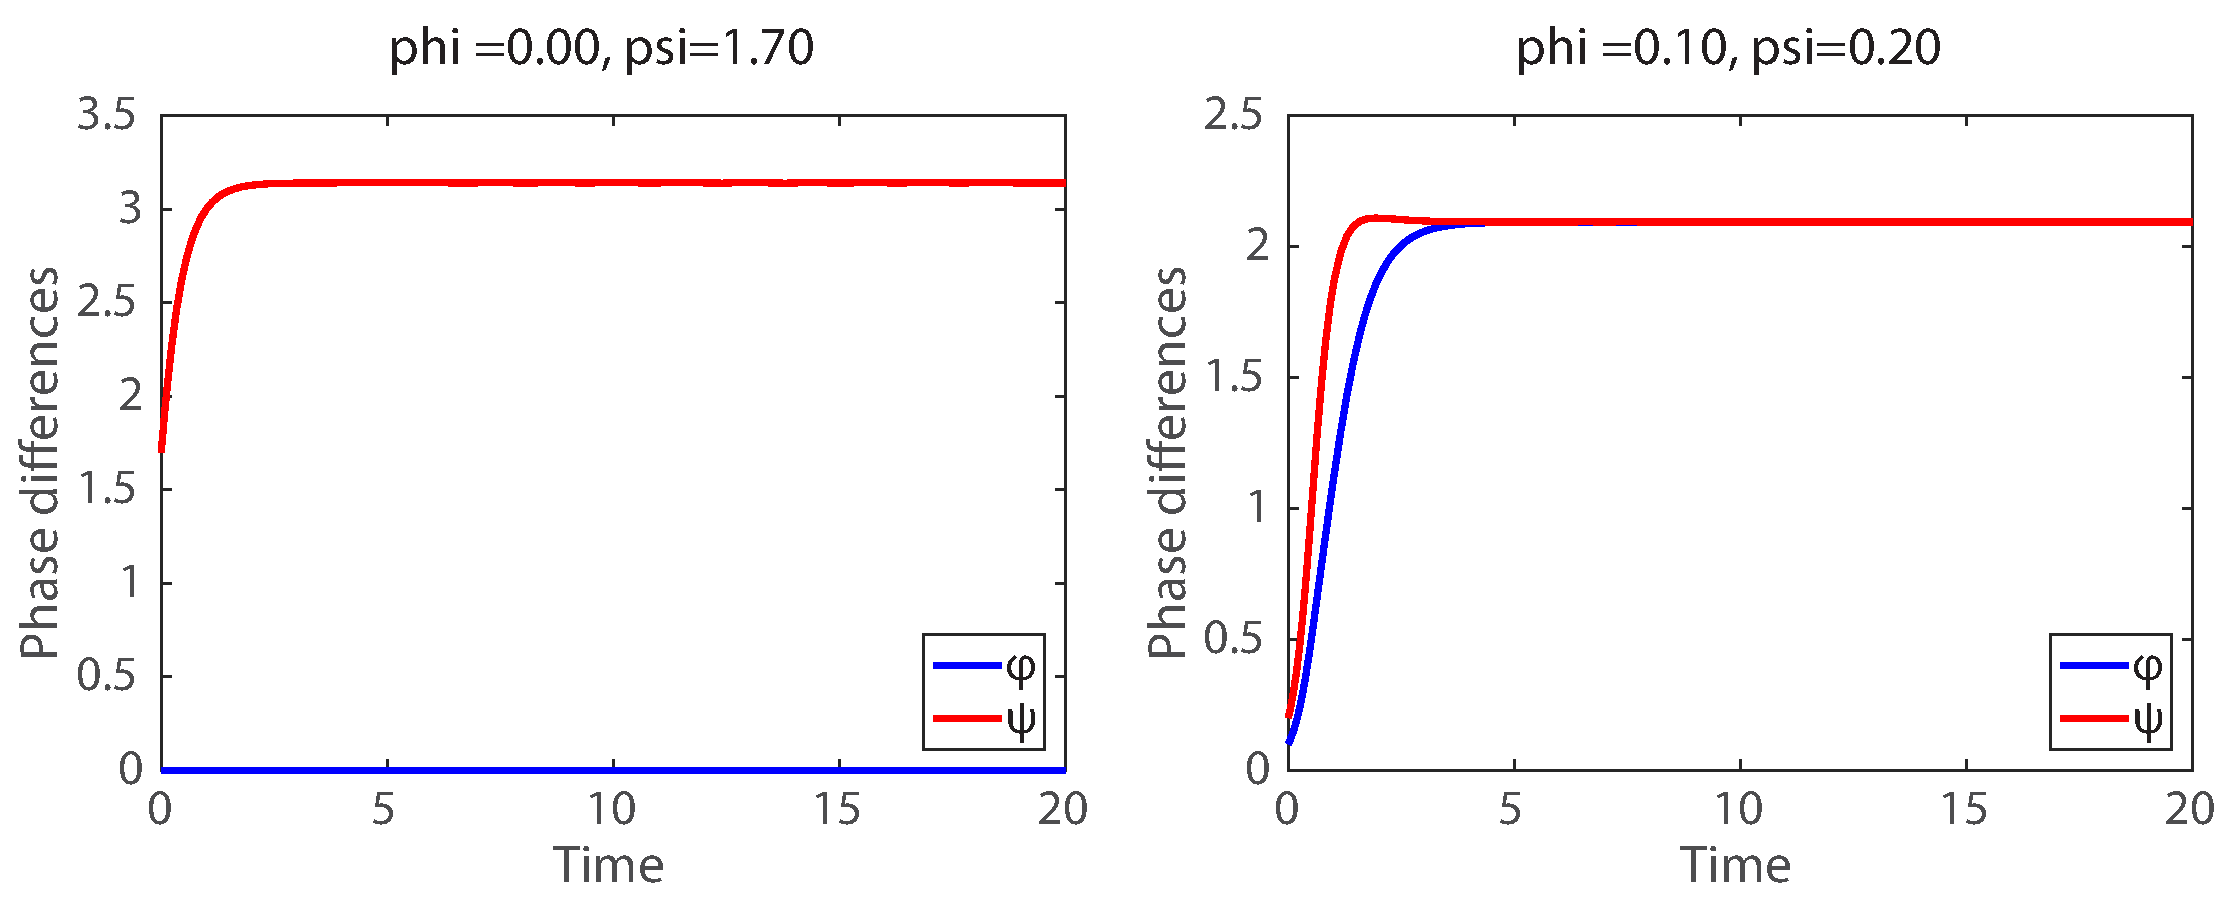
\includegraphics[width=0.7\textwidth]{frogs.pdf}
\caption{Timecourse of $\phi=\theta_2 - \theta_1$ and $\psi = \theta_3 - \theta_2$ for $a=-1$, $b=-1$ and (left) $\phi(0) = 0$ and $\psi(0) = 1.7$ or (right) $\phi(0)=0.1$ and $\psi(0) = 0.2$.}
\end{center}
\end{figure}
\begin{itemize}
\item If we perturb the phase of one frog, the system will tend to restore its relative phase (unless the perturbation is so large that the system approaches the other stable solution).
\item Similar models can also explain synchronization between coupled oscillators with slightly different frequencies. Some fireflies, for example, can sync to artificial light pulses with $\pm$15\% differences in period. (Fireflies of one species can even tune their baseline frequency for improved long-term matching.)
\item In this case the coupling was negative (driving the frog's timing apart), but for positive coupling we'd expect synchronization and stabilization of phase.
\end{itemize}


\section*{\textit{Dictyostelium discoideum} aggregation}

\begin{itemize}

\item Another example of a system of coupled oscillators is a cellular slime mold community coordinating aggregation. While the phase of this clock does not appear to be linked to an external environmental cue, individual cells can entrain on the extracellular products of already-oscillating neighbors, establishing synchrony between cells in the population.
\item \textit{Dictyostelium} normally live as individual amoebae, but when they begin to run out of food, these amoeba aggregate together to form a motile slug that can travel much faster than any cell alone. The goal of this movement is for the cells to reach a position from which their spores could be disbursed, hopefully to germinate in more favorable conditions. The slug is capable of traveling a few millimeters upward through the leaf litter, where it forms an upright stalk, at the tip of which will form a ball of spores.
\item One issue with this life strategy is that it requires cells to signal to one another that they are starving, identify the center of their community, and move toward that point to form an aggregate. 
\item The major chemical player in communication between cells in this system is cAMP. The external concentration of cAMP is found to oscillate in aggregating populations, and with each peak, cells exhibit contractions toward the center of the group.
\item After each peak, both intracellular and extracellular cAMP are hydrolyzed. Inside the cell, this process is carried out by the phosphodiesterase REG A.
\item When cAMP is added exogenously at the incorrect phase of the cycle, the phase is shifted; when it is continuously kept high, the cycle is eliminated entirely.
\item Cells detect cAMP through a high affinity receptor called CAR1. There are two main effects of signalling through CAR1: activation of ACA, an adenylyl cyclase, and activation of ERK2, which inhibits REG A.
\end{itemize}
\begin{figure}
\begin{center}
\includegraphics[width=0.5\textwidth]{maeda.png}
\caption{cAMP-based oscillator in \textit{Dictyostelium}, from Maeda 2004.}
\end{center}
\end{figure}
\begin{itemize}
\item What I have described so far is a positive feedback loop that would tend to increase intra- and extracellular cAMP indefinitely. The negative feedback loop in this case is that cAMP activates a protein called protein kinase A (PKA), which represses both ERK2 and ACA.
\item The following set of differential equations, modified from Laub and Loomis (1998) by Maeda et al. (2004), produce an oscillating system for an appropriate choice of parameter values:

\begin{eqnarray*}
\frac{d [\textrm{ACA}]}{dt} & = & k_1  [\textrm{CAR1}] - k_2 [\textrm{PKA}]  [\textrm{ACA}]\\
\frac{d [\textrm{PKA}]}{dt} & = & k_3  [\textrm{cAMPint}] - k_4 [\textrm{PKA}] \\
\frac{d[ \textrm{ERK2}]}{dt} & = & k_5  [\textrm{CAR1}] - k_6 [\textrm{PKA}]  [\textrm{ERK2}]\\
\frac{d [\textrm{REG A}]}{dt} & = & k_7  - k_8 [\textrm{REG A}]  [\textrm{ERK2}]\\
\frac{d [\textrm{cAMPint}]}{dt} & = & k_9  [\textrm{ACA}] - k_{10} [\textrm{REG A}] [\textrm{cAMPint}]\\
\frac{d[ \textrm{cAMPext}]}{dt} & = & k_{11}  [\textrm{ACA}] - k_{12}  [\textrm{cAMPext}]\\
\frac{d [\textrm{CAR1}]}{dt} & = & k_{13}  [\textrm{cAMPext}]  - k_{14} [\textrm{CAR1}] \\
\end{eqnarray*}

\end{itemize}

\begin{center}
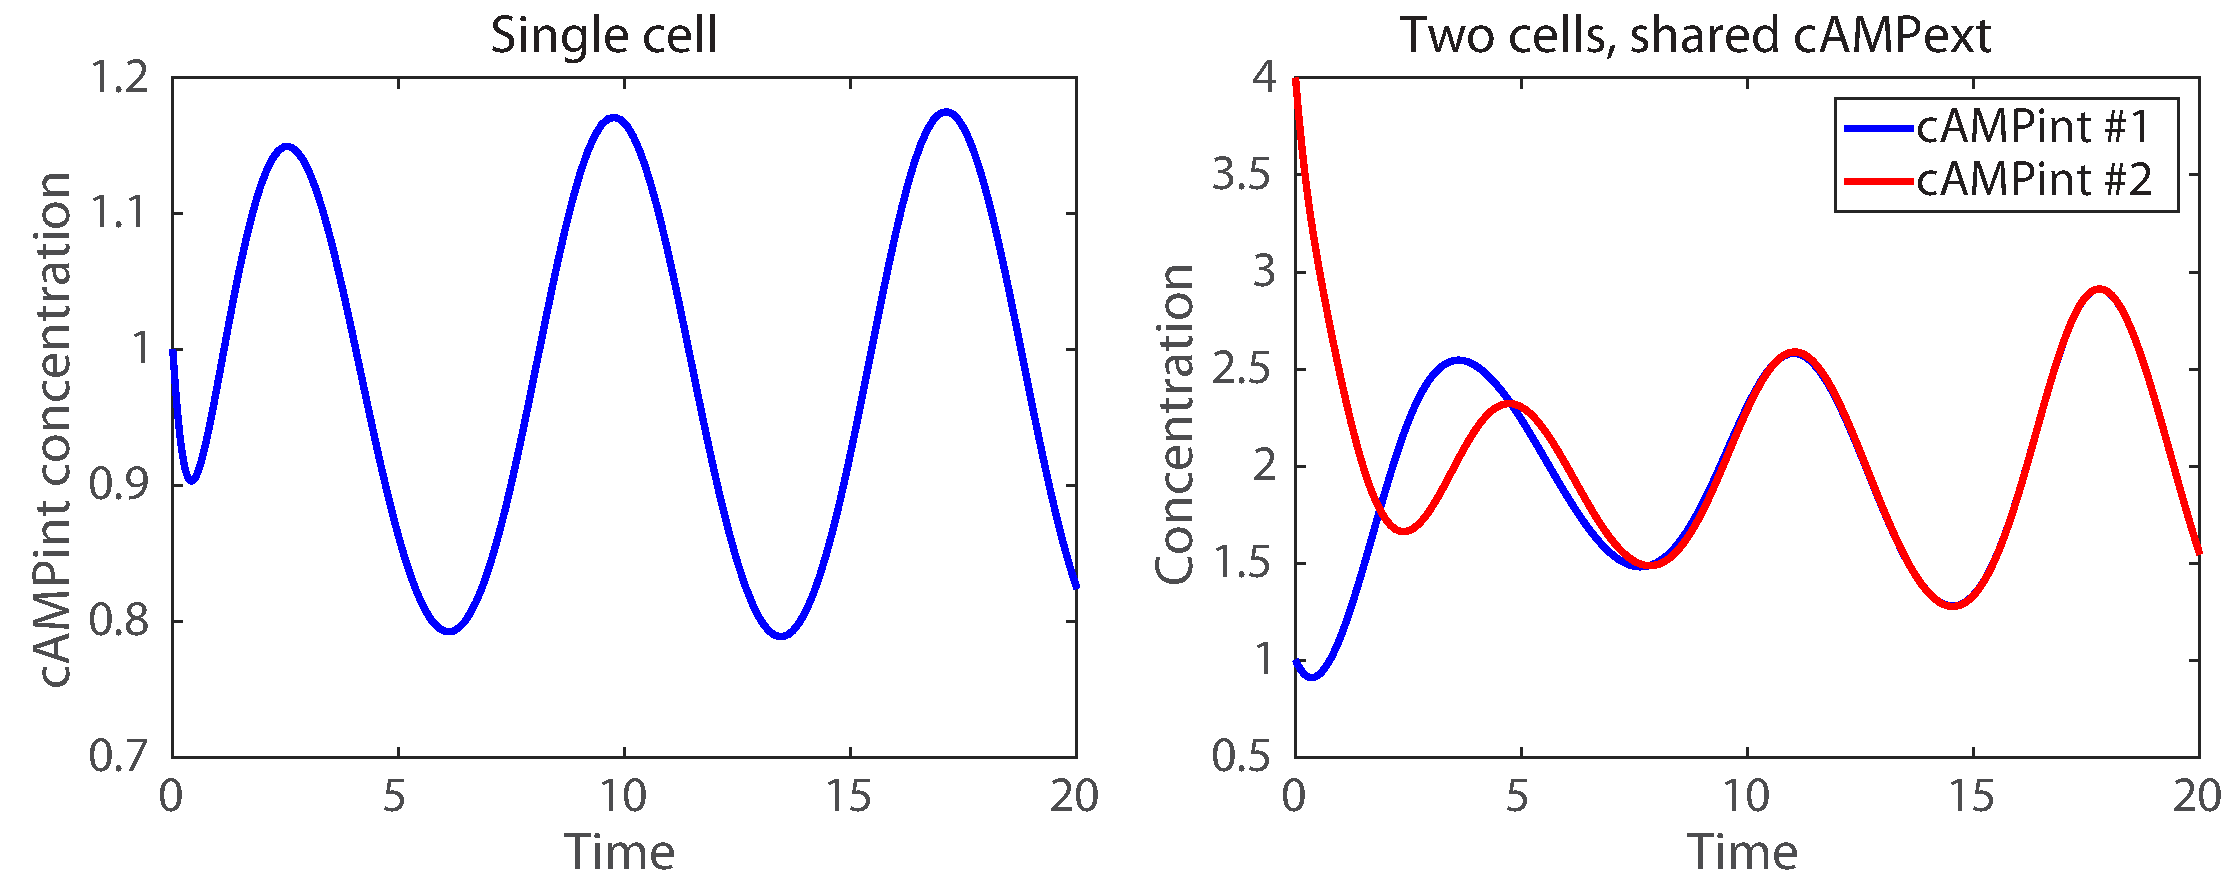
\includegraphics[width=0.7\textwidth]{slime.pdf}
\end{center}

\begin{itemize}

\item Although neighboring cells can phase-lock, on the larger scale of the population, moving fronts of external cAMP appear, ultimately forming spirals. Cells within the field of one spiral will ultimately form a slug together.
\item External cAMP also binds to a different G protein receptor to ultimately activate phospholipase C, which will produce IP$_3$, causing calcium oscillations that lead to directional pseudopod extension.
\end{itemize}

\section*{Summary}

\begin{itemize}
\item When we return after break, we'll continue our discussion of clocks and oscillations, launching into natural clocks whose oscillators depend on transcriptional feedback loops.
\item A majority of synthetic clocks rely on such feedback loops, which have been easier to construct than protein-protein interactions.
\item However, you will see that coupling has also been used to synchronize synthetic clocks such as the one developed in Jeff Hasty's group at UCSD.
\end{itemize}

\end{document}